
\bta{2012}



\section{Use of English}

\noindent
\textbf{Directions:}\\
Read the following text. Choose the best word (s) for each
	numbered blank and mark A, B, C or D on \textbf{ANSWER SHEET 1}.  (10 points)



\TiGanSpace


The ethical judgments of the Supreme Court justices have become an
important issue recently. The court cannot \cloze its
legitimacy as guardian of the rule of law \cloze justices
behave like politicians. Yet, in several instances, justices acted in
ways that \cloze the court's reputation for being independent
and impartial.

Justice Antonin Scalia, for example, appeared at political events. That
kind of activity makes it less likely that the court's decisions will
be \cloze as impartial judgments. Part of the problem is that
the justices are not \cloze by an ethics code. At the very
least, the court should make itself \cloze to the code of
conduct that \cloze to the rest of the federal judiciary.

This and other similar cases \cloze the question of whether
there is still a \cloze between the court and politics.

The framers of the Constitution envisioned law \cloze having
authority apart from politics. They gave justices permanent positions
\cloze they would be free to \cloze those in power
and have no need to \cloze political support. Our legal system
was designed to set law apart from politics precisely because they are
so closely \cloze.

Constitutional law is political because it results from choices rooted
in fundamental social \cloze like liberty and property. When
the court deals with social policy decisions, the law it \cloze
is inescapably political---which is why decisions split along
ideological lines are so easily \cloze as unjust.

The justices must \cloze doubts about the court's legitimacy
by making themselves \cloze to the code of conduct. That would
make their rulings more likely to be seen as separate from politics and,
\cloze , convincing as law.


\newpage

\begin{enumerate}
	%\renewcommand{\labelenumi}{\arabic{enumi}.}
	% A(\Alph) a(\alph) I(\Roman) i(\roman) 1(\arabic)
	%设定全局标号series=example	%引用全局变量resume=example
	%[topsep=-0.3em,parsep=-0.3em,itemsep=-0.3em,partopsep=-0.3em]
	%可使用leftmargin调整列表环境左边的空白长度 [leftmargin=0em]
	\item


\fourchoices
{emphasize}
{maintain}
{modify}
{recognize}




\item


\fourchoices
{when}
{lest}
{before}
{unless}




\item


\fourchoices
{restored}
{weakened}
{established}
{eliminated}




\item


\fourchoices
{challenged}
{compromised}
{suspected}
{accepted}




\item


\fourchoices
{advanced}
{caught}
{bound}
{founded}




\item


\fourchoices
{resistant}
{subject}
{immune}
{prone}




\item


\fourchoices
{resorts}
{sticks}
{leads}
{applies}




\item


\fourchoices
{evade}
{raise}
{deny}
{settle}




\item


\fourchoices
{line}
{barrier}
{similarity}
{conflict}




\item


\fourchoices
{by}
{as}
{through}
{towards}




\item


\fourchoices
{so}
{since}
{provided}
{though}




\item


\fourchoices
{serve}
{satisfy}
{upset}
{replace}




\item


\fourchoices
{confirm}
{express}
{cultivate}
{offer}




\item


\fourchoices
{guarded}
{followed}
{studied}
{tied}




\item


\fourchoices
{concepts}
{theories}
{divisions}
{conventions}




\item


\fourchoices
{excludes}
{questions}
{shapes}
{controls}




\item


\fourchoices
{dismissed}
{released}
{ranked}
{distorted}




\item


\fourchoices
{suppress}
{exploit}
{address}
{ignore}




\item


\fourchoices
{accessible}
{amiable}
{agreeable}
{accountable}




\item


\fourchoices
{by all means}
{at all costs}
{in a word}
{as a result}


\end{enumerate}


\vfil

\section{Reading Comprehension}


\noindent
\textbf{Part A}\\
\textbf{Directions:}\\
Read the following four texts. Answer the questions below each
	text by choosing A, B, C or
	D. Mark your answers on \textbf{ANSWER SHEET 1}. (40
	points)

\newpage
\subsection{Text 1}


Come on---Everybody's doing it. That whispered message, half
invitation and half forcing, is what most of us think of when we hear
the words \emph{peer pressure.} It usually leads to no good---drinking, drugs and casual sex.
But in her new book \emph{Join the Club}, Tina Rosenberg contends that peer pressure can also be a positive
force through what she calls the social cure, in which organizations and
officials use the power of group dynamics to help individuals improve
their lives and possibly the world.

Rosenberg, the recipient of a Pulitzer Prize, offers a host of examples
of the social cure in action: In South Carolina, a state-sponsored
antismoking program called Rage Against the Haze sets out to make
cigarettes uncool. In South Africa, an HIV-prevention initiative known
as loveLife recruits young people to promote safe sex among their peers.

The idea seems promising, and Rosenberg is a perceptive observer. Her
critique of the lameness of many public-health campaigns is
spot-on: they fail to mobilize peer pressure for healthy habits, and
they demonstrate a seriously flawed understanding of psychology. ``Dare
to be different, please don't smoke!'' pleads one billboard campaign
aimed at reducing smoking among teenagers---teenagers, who desire
nothing more than fitting in. Rosenberg argues convincingly that
public-health advocates ought to take a page from advertisers, so
skilled at applying peer pressure.

But on the general effectiveness of the social cure, Rosenberg is less
persuasive. \emph{Join the Club} is filled with too much irrelevant
detail and not enough exploration of the social and biological factors
that make peer pressure so powerful. The most glaring flaw of the social
cure as it's presented here is that it doesn't work very well for very
long. Rage Against the Haze failed once state funding was cut. Evidence
that the loveLife program produces lasting changes is limited and mixed.

There's no doubt that our peer groups exert enormous influence on our
behavior. An emerging body of research shows that positive health habits---as well as negative ones---spread through networks of friends via
social communication. This is a subtle form of peer pressure: we
unconsciously imitate the behavior we see every day.

Far less certain, however, is how successfully experts and bureaucrats
can select our peer groups and steer their activities in virtuous
directions. It's like the teacher who breaks up the troublemakers in the
back row by pairing them with better-behaved classmates. The tactic
never really works. And that's the problem with a social cure engineered
from the outside: in the real world, as in school, we insist on choosing
our own friends.

\begin{enumerate}[resume]
	%\renewcommand{\labelenumi}{\arabic{enumi}.}
	% A(\Alph) a(\alph) I(\Roman) i(\roman) 1(\arabic)
	%设定全局标号series=example	%引用全局变量resume=example
	%[topsep=-0.3em,parsep=-0.3em,itemsep=-0.3em,partopsep=-0.3em]
	%可使用leftmargin调整列表环境左边的空白长度 [leftmargin=0em]
	\item
According to the first
paragraph, peer pressure often emerges as \lineread.


\fourchoices
{a supplement to the social cure}
{a stimulus to group dynamics}
{an obstacle to social progress}
{a cause of undesirable behaviors}


\item
Rosenberg holds that public advocates should \lineread.


\fourchoices
{recruit professional advertisers}
{learn from advertisers' experience}
{stay away from commercial advertisers}
{recognize the limitations of advertisements}



\item
 In the author's view, Rosenberg's book fails to \lineread.


\fourchoices
{adequately probe social and biological factors}
{effectively evade the flaws of the social cure}
{illustrate the functions of state funding}
{produce a long-lasting social effect}


\item
Paragraph 5 shows that our imitation of behaviors \lineread.


\fourchoices
{is harmful to our networks of friends}
{will mislead behavioral studies}
{occurs without our realizing it}
{can produce negative health habits}


\item
 The author suggests in the last paragraph that the effect
ofpeer pressure is \lineread.



\fourchoices
{harmful}
{desirable}
{profound}
{questionable}

\end{enumerate}



\newpage
\subsection{Text 2}


A deal is a deal---except, apparently, when Entergy is involved. The
company, a major energy supplier in New England, provoked justified
outrage in Vermont last week when it announced it was
\uline{reneging on} a longstanding commitment to abide by the strict
nuclear regulations.

Instead, the company has done precisely what it had long promised it
would not: challenge the constitutionality of Vermont's rules in the
federal court, as part of a desperate effort to keep its Vermont Yankee
nuclear power plant running. It's a stunning move.

The conflict has been surfacing since 2002, when the corporation bought
Vermont's only nuclear power plant, an aging reactor in Vernon. As a
condition of receiving state approval for the sale, the company agreed
to seek permission from state regulators to operate past 2012. In 2006,
the state went a step further, requiring that any extension of the
plant's license be subject to Vermont legislature's approval. Then, too,
the company went along.

Either Entergy never really intended to live by those commitments, or it
simply didn't foresee what would happen next. A string of accidents,
including the partial collapse of a cooling tower in 2007 and the
discovery of an underground pipe system leakage, raised serious
questions about both Vermont Yankee's safety and Entergy's management---especially after the company made misleading statements about the
pipe. Enraged by Entergy's behavior, the Vermont Senate voted 26 to 4
last year against allowing an extension.

Now the company is suddenly claiming that the 2002 agreement is invalid
because of the 2006 legislation, and that only the federal government
has regulatory power over nuclear issues. The legal issues in the case
are obscure: whereas the Supreme Court has ruled that states do have
some regulatory authority over nuclear power, legal scholars say that
Vermont case will offer a precedent-setting test of how far those powers
extend. Certainly, there are valid concerns about the patchwork
regulations that could result if every state sets its own rules. But had
Entergy kept its word, that debate would be beside the point.

The company seems to have concluded that its reputation in Vermont is
already so damaged that it has nothing left to lose by going to war with
the state. But there should be consequences. Permission to run a nuclear
plant is a public trust. Entergy runs 11 other reactors in the United
States, including Pilgrim Nuclear station in Plymouth. Pledging to run
Pilgrim safely, the company has applied for federal permission to keep
it open for another 20 years. But as the Nuclear Regulatory Commission
(NRC) reviews the company's application, it should keep it mind what
promises from Entergy are worth.

\begin{enumerate}[resume]
	%\renewcommand{\labelenumi}{\arabic{enumi}.}
	% A(\Alph) a(\alph) I(\Roman) i(\roman) 1(\arabic)
	%设定全局标号series=example	%引用全局变量resume=example
	%[topsep=-0.3em,parsep=-0.3em,itemsep=-0.3em,partopsep=-0.3em]
	%可使用leftmargin调整列表环境左边的空白长度 [leftmargin=0em]
	\item
The phrase ``reneging on'' (Line 3. para. 1) is closest in
meaning to \lineread.


\fourchoices
{condemning}
{reaffirming}
{dishonoring}
{securing}



\item
By entering into the 2002 agreement, Entergy intended to \lineread.


\fourchoices
{obtain protection from Vermont regulators}
{seek favor from the federal legislature}
{acquire an extension of its business license}
{get permission to purchase a power plant}


\item
According to Paragraph 4, Entergy seems to have problems
with its \lineread.


\fourchoices
{managerial practices}
{technical innovativeness}
{financial goals}
{business vision}



\item
 In the author's view, the Vermont case will test \lineread.


\fourchoices
{Entergy's capacity to fulfill all its promises}
{the mature of states' patchwork regulations}
{the federal authority over nuclear issues}
{the limits of states' power over nuclear issues}



\item
It can be inferred from the last paragraph that \lineread.


\fourchoices
{Entergy's business elsewhere might be affected}
{the authority of the NRC will be defied}
{Entergy will withdraw its Plymouth application}
{Vermont's reputation might be damaged}

	
\end{enumerate}



\newpage
\subsection{Text 3}


In the idealized version of how science is done, facts about the world
are waiting to be observed and collected by objective researchers who
use the scientific method to carry out their work. But in the everyday
practice of science, discovery frequently follows an ambiguous and
complicated route. We aim to be objective, but we cannot escape the
context of our unique life experiences. Prior knowledge and interests
influence what we experience, what we think our experiences mean, and
the subsequent actions we take. Opportunities for misinterpretation,
error, and self-deception abound.

Consequently, discovery claims should be thought of as protoscience.
Similar to newly staked mining claims, they are full of potential. But
it takes collective scrutiny and acceptance to transform a discovery
claim into a mature discovery. This is the credibility process, through
which the individual researcher's \emph{me}, \emph{here}, \emph{now} becomes the community's
\emph{anyone}, \emph{anywhere}, \emph{anytime}. Objective knowledge is the goal, not the
starting point.

Once a discovery claim becomes public, the discoverer receives
intellectual credit. But, unlike with mining claims, the community takes
control of what happens next. Within the complex social structure of the
scientific community, researchers make discoveries; editors and
reviewers act as gatekeepers by controlling the publication process;
other scientists use the new finding to suit their own purposes; and
finally, the public (including other scientists) receives the new
discovery and possibly accompanying technology. As a discovery claim
works its way through the community, the interaction and confrontation
between shared and competing beliefs about the science and the
technology involved transforms an individual's discovery claim into the
community's credible discovery.

Two paradoxes exist throughout this credibility process. First,
scientific work tends to focus on some aspect of prevailing knowledge
that is viewed as incomplete or incorrect. Little reward accompanies
duplication and confirmation of what is already known and believed. The
goal is \emph{new-search}, not \emph{re-search.} Not surprisingly, newly
published discovery claims and credible discoveries that appear to be
important and convincing will always be open to challenge and potential
modification or refutation by future researchers. Second, novelty itself
frequently provokes disbelief. Nobel Laureate and physiologist Albert
Szent-Györgyi once described discovery as ``seeing what everybody has
seen and thinking what nobody has thought.'' But thinking what nobody
else has thought and telling others what they have missed may not change
their views. Sometimes years are required for truly novel discovery
claims to be accepted and appreciated.

In the end, credibility ``happens'' to a discovery claim---a process
that corresponds to what philosopher Annette Baier has described as
the \emph{commons of the mind}. ``We reason together, challenge, revise, and
complete each other's reasoning and each other's conceptions of
reason.''

\begin{enumerate}[resume]
	%\renewcommand{\labelenumi}{\arabic{enumi}.}
	% A(\Alph) a(\alph) I(\Roman) i(\roman) 1(\arabic)
	%设定全局标号series=example	%引用全局变量resume=example
	%[topsep=-0.3em,parsep=-0.3em,itemsep=-0.3em,partopsep=-0.3em]
	%可使用leftmargin调整列表环境左边的空白长度 [leftmargin=0em]
	\item
According to the first paragraph, the process of discovery
is characterized by its \lineread.


\fourchoices
{uncertainty and complexity}
{misconception and deceptiveness}
{logicality and objectivity}
{systematicness and regularity}


\item
It can be inferred from Paragraph 2 that credibility process
requires \lineread.


\fourchoices
{strict inspection}
{shared efforts}
{individual wisdom}
{persistent innovation}



\item
Paragraph 3 shows that a discovery claim becomes credible
after it \lineread.


\fourchoices
{has attracted the attention of the general public}
{has been examined by the scientific community}
{has received recognition from editors and reviewers}
{has been frequently quoted by peer scientists}


\item
Albert Szent-Györgyi would most likely agree that \lineread.


\fourchoices
{scientific claims will survive challenges}
{discoveries today inspire future research}
{efforts to make discoveries are justified}
{scientific work calls for a critical mind}


\item
Which of the following would be the best title of the text?


\fourchoices
{Novelty as an Engine of Scientific Development}
{Collective Scrutiny in Scientific Discovery}
{Evolution of Credibility in Doing Science}
{Challenge to Credibility at the Gate to Science}

\end{enumerate}


\newpage
\subsection{Text 4}


If the trade unionist Jimmy Hoffa were alive today, he would probably
represent civil servants. When Hoffa's Teamsters were in their prime in
1960, only one in ten American government workers belonged to a union;
now 36\% do. In 2009 the number of unionists in America's public sector
passed that of their fellow members in the private sector. In Britain,
more than half of public-sector workers but only about 15\% of
private-sector ones are unionized.

There are three reasons for the public-sector unions' thriving. First,
they can shut things down without suffering much in the way of
consequences. Second, they are mostly bright and well-educated. A
quarter of America's public-sector workers have a university degree.
Third, they now dominate left--of--centre politics. Some of their ties go
back a long way. Britain's Labor Party, as its name implies, has long
been associated with trade unionism. Its current leader, Ed Miliband,
owes his position to votes from public--sector unions.

At the state level their influence can be even more fearsome. Mark
Baldassare of the Public Policy Institute of California points out that
much of the state's budget is patrolled by unions. The teachers' unions
keep an eye on schools, the CCPOA on prisons and a variety of labor
groups on health care.

In many rich countries average wages in the state sector are higher than
in the private one. But the real gains come in benefits and work
practices. Politicians have repeatedly ``backloaded'' public-sector pay
deals, keeping the pay increases modest but adding to holidays and
especially pensions that are already generous.

Reform has been vigorously opposed, perhaps most egregiously in
education, where charter schools, academies and merit pay all faced
drawn-out battles. Even though there is plenty of evidence that the
quality of the teachers is the most important variable, teachers' unions
have fought against getting rid of bad ones and promoting good ones.

As the cost to everyone else has become clearer, politicians have begun
to clamp down. In Wisconsin the unions have rallied thousands of
supporters against Scott Walker, the hardline Republican governor. But
many within the public sector suffer under the current system, too.

John Donahue at Harvard's Kennedy School points out that the norms of
culture in Western civil services suit those who want to stay put but is
bad for high achievers. The only American public-sector workers who earn
well above \$250, 000 a year are university sports coaches and the
president of the United States. Bankers' fat pay packets have attracted
much criticism, but a public-sector system that does not reward high
achievers may be a much bigger problem for America.

\begin{enumerate}[resume]
	%\renewcommand{\labelenumi}{\arabic{enumi}.}
	% A(\Alph) a(\alph) I(\Roman) i(\roman) 1(\arabic)
	%设定全局标号series=example	%引用全局变量resume=example
	%[topsep=-0.3em,parsep=-0.3em,itemsep=-0.3em,partopsep=-0.3em]
	%可使用leftmargin调整列表环境左边的空白长度 [leftmargin=0em]
	\item
 It can be learned from the first paragraph that \lineread.


\fourchoices
{Teamsters still have a large body of members}
{Jimmy Hoffa used to work as a civil servant}
{unions have enlarged their public-sector membership}
{the government has improved its relationship with unionists}



\item
Which of the following is true of Paragraph 2?


\fourchoices
{Public-sector unions are prudent in taking actions.}
{Education is required for public-sector union membership.}
{Labor Party has long been fighting against public-sector unions.}
{Public-sector unions seldom get in trouble for their actions.}



\item
It can be learned from Paragraph 4 that the income in the
state sector is \lineread.


\fourchoices
{illegally secured}
{indirectly augmented}
{excessively increased}
{fairly adjusted}



\item
The example of the unions in Wisconsin shows that unions \lineread.


\fourchoices
{often run against the current political system}
{can change people's political attitudes}
{may be a barrier to public-sector reforms}
{are dominant in the government}


\item
John Donahue's attitude towards the public-sector system is
one of \lineread.


\fourchoices
{disapproval}
{appreciation}
{tolerance}
{indifference}


	
\end{enumerate}


\newpage
\noindent
\textbf{Part B}\\
\textbf{Directions:}\\
In the following text, some sentences have been removed. For
	Questions 41-45, choose the most suitable one from the list A-G to fit
	into each of the numbered blanks. There are two extra choices, which do
	not fit in any of the blanks. Mark your answers on \textbf{ANSWER SHEET 1}. (10
	points)



\TiGanSpace

Think of those fleeting moments when you look out of an aeroplane window
and realise that you are flying, higher than a bird. Now think of your
laptop, thinner than a brown-paper envelope, or your cellphone in the
palm of your hand. Take a moment or two to wonder at those marvels. You
are the lucky inheritor of a dream come true.

The second half of the 20th century saw a collection of geniuses,
warriors, entrepreneurs and visionaries labour to create a fabulous
machine that could function as a typewriter and printing press, studio
and theatre, paintbrush and gallery, piano and radio, the mail as well
as the mail carrier. \linefill.

The networked computer is an amazing device, the first media machine
that serves as the mode of production, means of distribution, site of
reception, and place of praise and critique. The computer is the 21 st
century's culture machine.

But for all the reasons there are to celebrate the computer, we must
also act with caution. \linefill. I call it a secret
war for two reasons. First, most people do not realise that there are
strong commercial agendas at work to keep them in passive consumption
mode. Second, the majority of people who use networked computers to
upload are not even aware of the significance of what they are doing.

All animals download, but only a few upload. Beavers build dams and
birds make nests. Yet for the most part, the animal kingdom moves
through the world downloading. Humans are unique in their capacity to
not only make tools but then turn around and use them to create
superfluous material goods--- paintings, sculpture and
architecture --- and superfluous experiences ---music, literature,
religion and philosophy. \linefill.

For all the possibilities of our new culture machines, most people are
still stuck in download mode. Even after the advent of widespread social
media, a pyramid of production remains, with a small number of people
uploading material, a slightly larger group commenting on or modifying
that content, and a huge percentage remaining content to just consume.
\linefill.

Television is a one-way tap flowing into our homes. The hardest task
that television asks of anyone is to turn the power off after he has
turned it on. \linefill.

What counts as meaningful uploading? My definition revolves around the
concept of  ``stickiness''---creations and experiences to which others
adhere.

\begin{listmatch}
	%\renewcommand{\labelenumi}{\arabic{enumi}.}
	% A(\Alph) a(\alph) I(\Roman) i(\roman) 1(\arabic)
	%设定全局标号series=example	%引用全局变量resume=example
	%[topsep=-0.3em,parsep=-0.3em,itemsep=-0.3em,partopsep=-0.3em]
	%可使用leftmargin调整列表环境左边的空白长度 [leftmargin=0em]
	\item
 Of course, it is precisely these superfluous things that define
human culture and ultimately what it is to be human. Downloading and
consuming culture requires great skills, but failing to move beyond
downloading is to strip oneself of a defining constituent of humanity.


\item 
Applications like tumblr. com, which allow users to combine
pictures, words and other media in creative ways and then share them,
have the potential to add stickiness by amusing, entertaining and
enlightening others.


\item 
Not only did they develop such a device but by the turn of the
millennium they had also managed to embed it in a worldwide system
accessed by billions of people every day.


\item 
This is because the networked computer has sparked a secretwar
between downloading and uploading---between passive consumption and
active creation---whose outcome will shape our collective future in
ways we can only begin to imagine.


\item 
The challenge the computer mounts to television thus bears
little similarity to one format being replaced by another in the manner
of record players being replaced by CD players.


\item 
One reason for the persistence of this pyramid of production is
that for the past half-century, much of the world's media culture has
been defined by a single medium---television---and television is
defined by downloading.


\item 
The networked computer offers the first chance in 50 years to
reverse the flow, to encourage thoughtful downloading and, even more
importantly, meaningful uploading.
\end{listmatch}


\newpage
\noindent
\textbf{Part C}\\
\textbf{Directions:}\\
Read the following text carefully and then translate the
	underlined segments into Chinese. Your translation should be written
	clearlyon \textbf{ANSWER SHEET 2}. (10 points)



\TiGanSpace


Since the days of Aristotle, a search for universal principles has
characterized the scientific enterprise. In some ways, this quest for
commonalities defines science. Newton's laws of motion and Darwinian
evolution each bind a host of different phenomena into a single
explicatory framework.

\transnum \uline{In physics, one approach takes this impulse for
	unification to its extreme, and seeks a theory of everything---a
	single generative equation for all we see.} It is becoming less clear,
however, that such a theory would be a simplification, given the
dimensions and universes that it might entail. Nonetheless, unification
of sorts remains a major goal.

This tendency in the natural sciences has long been evident in the
social sciences too. \transnum \uline{Here, Darwinism seems to offer
	justification, for if all humans share common origins, it seems
	reasonable to suppose that cultural diversity could also be traced to
	more constrained beginnings}. Just as the bewildering variety of human
courtship rituals might all be considered forms of sexual selection,
perhaps the world's languages, music, social and religious customs and
even history are governed by universal features. \transnum \uline{To
	filter out what is unique from what is shared might enable us to
	understand how complex cultural behavior arose and what guides it in
	evolutionary or cognitive terms}.

That, at least, is the hope. But a comparative study of linguistic
traits published online today supplies a reality check. Russell Gray at
the University of Auckland and his colleagues consider the evolution of
grammars in the light of two previous attempts to find universality in
language.

The most famous of these efforts was initiated by Noam Chomsky, who
suggested that humans are born with an innate language---acquisition
capacity that dictates a universal grammar. A few generative rules are
then sufficient to unfold the entire fundamental structure of a
language, which is why children can learn it so quickly.

\transnum \uline{The second, by Joshua Greenberg, takes a more empirical
	approach to universality, identifying traits (particularly in word
	order) shared by many language which are considered to represent biases
	that result from cognitive constraints}.

Gray and his colleagues have put them to the test by examining four
family trees that between them represent more than 2, 000 languages.
\transnum \uline{Chomsky's grammar should show patterns of language change
	that are independent of the family tree or the pathway tracked through
	it, whereas Greenbergian universality predicts strong co-dependencies
	between particular types of word-order relations.} Neither of these
patterns is borne out by the analysis, suggesting that the structures of
the languages are lineage-specific and not governed by universals.




\newpage


\section{Writing}


\noindent
\textbf{Part A}\\
\textbf{51. Directions:}

Some international students are coming to your university. Write them an
email in the name of the Students' Union to
\begin{listwrite}
	%\renewcommand{\labelenumi}{\arabic{enumi}.}
	% A(\Alph) a(\alph) I(\Roman) i(\roman) 1(\arabic)
	%设定全局标号series=example	%引用全局变量resume=example
	%[topsep=-0.3em,parsep=-0.3em,itemsep=-0.3em,partopsep=-0.3em]
	%可使用leftmargin调整列表环境左边的空白长度 [leftmargin=0em]
	\item
 extend your welcome and

\item 
provide some suggestions for their campus life here.
\end{listwrite}


You should write about 100 words on ANSWER SHEET 2.

\textbf{Do not} sign your own name at the end of the letter. Use ``Li
Ming'' instead.

\textbf{Do not} write the address. (10 points)


\vspace{2em}

\noindent
\textbf{Part B}\\
\textbf{52. Directions:}

Write an essay of 160-200 words based on the following drawing. In your
essay, you should
\begin{listwrite}
	%\renewcommand{\labelenumi}{\arabic{enumi}.}
	% A(\Alph) a(\alph) I(\Roman) i(\roman) 1(\arabic)
	%设定全局标号series=example	%引用全局变量resume=example
	%[topsep=-0.3em,parsep=-0.3em,itemsep=-0.3em,partopsep=-0.3em]
	%可使用leftmargin调整列表环境左边的空白长度 [leftmargin=0em]
	\item
describe the drawing briefly,

\item 
explain its intended meaning, and

\item 
 give your comments.
\end{listwrite}

You should write neatly on ANSWER SHEET 2. (20 points)



\begin{figure}[h!]
	\centering
	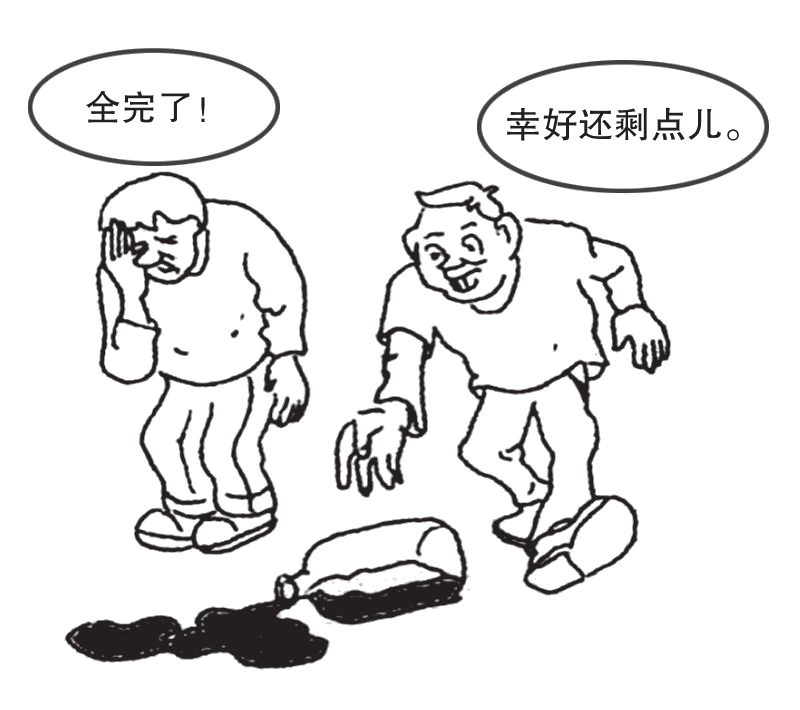
\includegraphics[width=0.45\linewidth]{picture/2012.png}
\end{figure}



